% Created 2016-08-17 Wed 14:38
\documentclass[tikz]{standalone}

\usepackage[utf8]{inputenc}
\usepackage[T1]{fontenc}
\usepackage{helvet}
\usepackage{../../templates/msc}

\renewcommand{\familydefault}{\sfdefault}

\tikzset{
every picture/.style={
line width=1pt
}}

\usepackage{tikz}
\author{Holger Karl}
\date{\today}
\title{}


\begin{document}
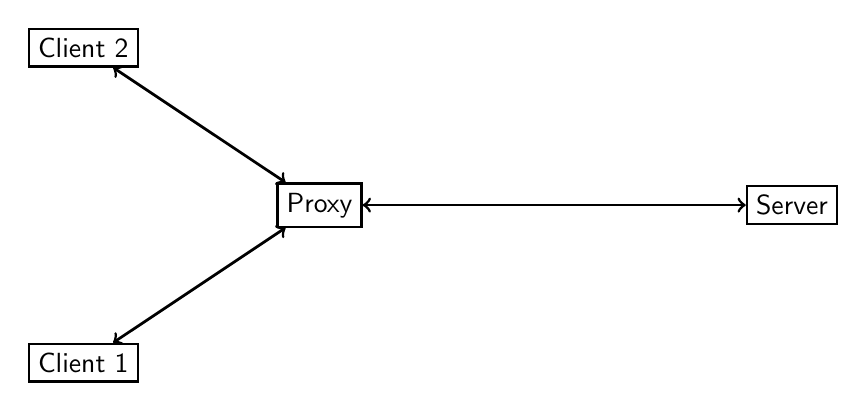
\begin{tikzpicture}[auto, xscale=3,
block/.style = {rectangle, draw=black, thick, align=left}]
\node[block] at (0,0) (c1) {Client 1};
\node[block] at (0,4) (c2) {Client 2}; 
\node[block] at (1,2) (pr) {Proxy}; 
\node[block] at (3,2) (s) {Server}; 
% \draw ([xshift=-0.5mm,yshift=-1mm]s1.south west) rectangle ([xshift=+0.5mm,yshift=+1mm]s3.north
% east);
% \node at (2,3.5) {Server group};
% \draw [->] (c1) -- ()
% \draw  (2,3) node[minimum width=4cm, minimum
% height=4cm,draw,label={Server group}] (sg) {};
\draw [<->] (c1) -- (pr); 
\draw [<->] (c2) -- (pr); 
\draw [<->] (pr) -- (s); 

\end{tikzpicture}
\end{document}